\documentclass{article}
\usepackage[margin=.5in]{geometry}
\usepackage{tikz}
\usetikzlibrary{shapes, arrows.meta} 
\usepackage{amsmath}

\begin{document}

\textbf{Exercice 3}

\vspace{0.5cm}

a)

\begin{center}
    \begin{minipage}{0.3\textwidth}
        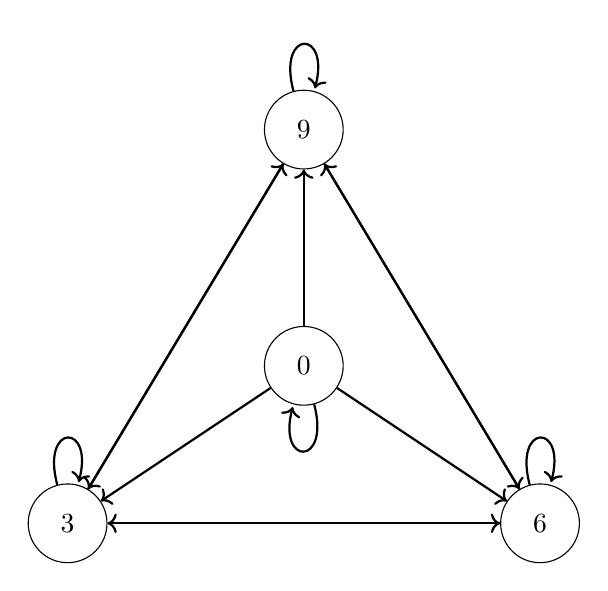
\begin{tikzpicture}
            \node[circle, draw, minimum size=1cm] (n0) at (0, 1) {0};
            \node[circle, draw, minimum size=1cm] (n3) at (-3, -1) {3};
            \node[circle, draw, minimum size=1cm] (n6) at (3, -1) {6};
            \node[circle, draw, minimum size=1cm] (n9) at (0, 4) {9}; 
            \draw[->, thick] (n0) edge[loop below] (n0);
            \draw[->, thick] (n3) edge[loop above] (n3);
            \draw[->, thick] (n6) edge[loop above] (n6);
            \draw[->, thick] (n9) edge[loop above] (n9);
            \draw[->, thick] (n0) -- (n3);
            \draw[->, thick] (n0) -- (n6);
            \draw[->, thick] (n0) -- (n9);
            \draw[->, thick] (n3) -- (n6);
            \draw[->, thick] (n6) -- (n3);
            \draw[->, thick] (n3) -- (n9);
            \draw[->, thick] (n9) -- (n3);
            \draw[->, thick] (n6) -- (n9);
            \draw[->, thick] (n9) -- (n6);
        \end{tikzpicture}
    \end{minipage}

    \begin{minipage}{0.3\textwidth}
        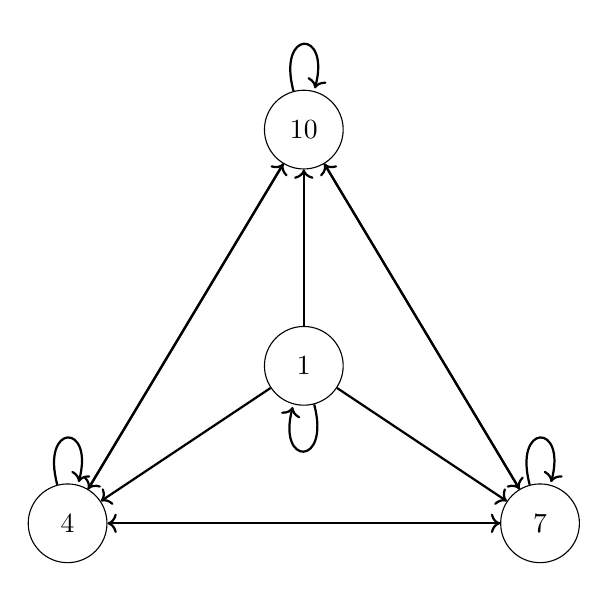
\begin{tikzpicture}
            \node[circle, draw, minimum size=1cm] (n1) at (0, 1) {1};
            \node[circle, draw, minimum size=1cm] (n4) at (-3, -1) {4};
            \node[circle, draw, minimum size=1cm] (n7) at (3, -1) {7};
            \node[circle, draw, minimum size=1cm] (n10) at (0, 4) {10}; 
            \draw[->, thick] (n1) edge[loop below] (n1);
            \draw[->, thick] (n4) edge[loop above] (n4);
            \draw[->, thick] (n7) edge[loop above] (n7);
            \draw[->, thick] (n10) edge[loop above] (n10);
            \draw[->, thick] (n1) -- (n4);
            \draw[->, thick] (n1) -- (n7);
            \draw[->, thick] (n1) -- (n10);
            \draw[->, thick] (n4) -- (n7);
            \draw[->, thick] (n7) -- (n4);
            \draw[->, thick] (n4) -- (n10);
            \draw[->, thick] (n10) -- (n4);
            \draw[->, thick] (n7) -- (n10);
            \draw[->, thick] (n10) -- (n7);
        \end{tikzpicture}
    \end{minipage}
    \hspace{4cm}
    \begin{minipage}{0.3\textwidth}
        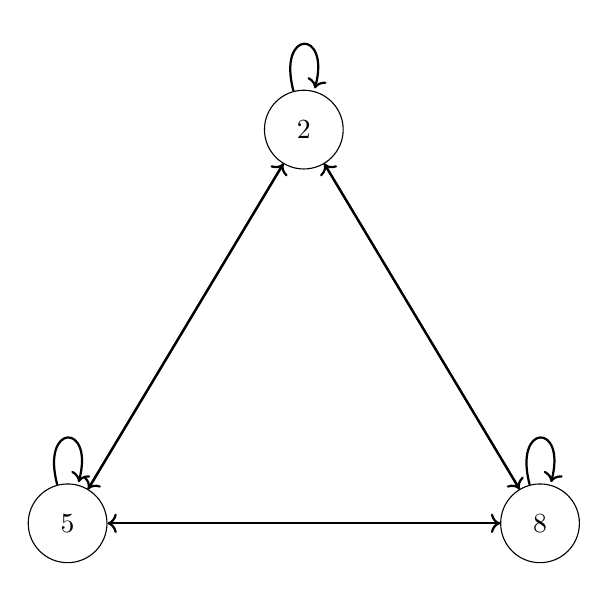
\begin{tikzpicture}
            \node[circle, draw, minimum size=1cm] (n5) at (-3, -1) {5};
            \node[circle, draw, minimum size=1cm] (n8) at (3, -1) {8};
            \node[circle, draw, minimum size=1cm] (n2) at (0, 4) {2}; 
            \draw[->, thick] (n5) edge[loop above] (n5);
            \draw[->, thick] (n8) edge[loop above] (n8);
            \draw[->, thick] (n2) edge[loop above] (n2);
            \draw[->, thick] (n2) -- (n5);
            \draw[->, thick] (n2) -- (n8);
            \draw[->, thick] (n5) -- (n2);
            \draw[->, thick] (n5) -- (n8);
            \draw[->, thick] (n8) -- (n2);
            \draw[->, thick] (n8) -- (n5);
        \end{tikzpicture}
    \end{minipage}
\end{center}

\vspace{0.5cm}

b) 
\begin{center}
    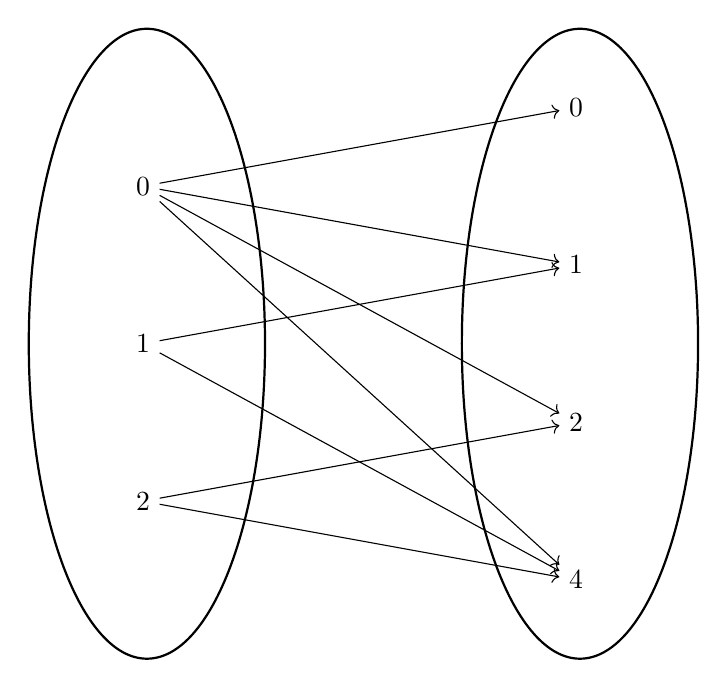
\begin{tikzpicture}
        \node (d0) at (-.8, 5) {0};
        \node (d1) at (-.8, 3) {1};
        \node (d2) at (-.8, 1) {2};

        \node (c0) at (4.7, 6) {0};
        \node (c1) at (4.7, 4) {1};
        \node (c2) at (4.7, 2) {2};
        \node (c4) at (4.7, 0) {4};
        
        \draw[->] (d0) -- (c0);
        \draw[->] (d0) -- (c1);
        \draw[->] (d0) -- (c2);
        \draw[->] (d0) -- (c4);
        \draw[->] (d1) -- (c1);
        \draw[->] (d1) -- (c4);
        \draw[->] (d2) -- (c2);
        \draw[->] (d2) -- (c4);

        \draw[solid, thick] (-0.75, 3) ellipse (1.50 and 4); 
        \draw[solid, thick] (4.75, 3) ellipse (1.50 and 4); 
    \end{tikzpicture}
\end{center}


\end{document}
